\documentclass[12pt]{extarticle}

\usepackage[utf8]{vietnam}
\usepackage{graphicx}
\usepackage{fancyhdr}
\usepackage{parskip}
\usepackage{amssymb}
\usepackage{amsmath}
\usepackage{float}
\usepackage{tikz}
\usepackage{fancybox}
\usetikzlibrary{positioning}
\usepackage[left=3 cm,right=3 cm,top=3cm,bottom=3cm]{geometry}
\usepackage[labelfont=bf]{caption}
\usepackage[hidelinks]{hyperref}
\usepackage{bookmark}
\usepackage{enumitem}
\usepackage[bottom]{footmisc}

\pagestyle{fancy}
\renewcommand{\sectionmark}[1]{\markboth{#1}{}} 
\fancyhf{}
\fancyhead[R]{\normalsize{\textit{\leftmark}}}
%\rhead{Phân giải đồng tham chiếu cho đối tượng và thuộc tính trong khai khoáng ý kiến}
\fancyhead[LE,LO]{\thepage}
%\fancyfoot[LE,RO]{\thepage} 
\renewcommand{\headrulewidth}{0.4pt}
%\renewcommand{\footrulewidth}{0.4pt}

\graphicspath{{images/}}

%-----------------SET PARAMS----------------------------------
\tikzset{
  treenode/.style = {shape=rectangle,
                     draw, align=center,
                     top color=white, bottom color=blue!20},
  root/.style     = {treenode, font=\Large, bottom color=red!30},
  env/.style      = {treenode, font=\ttfamily\normalsize},
  dummy/.style    = {circle,draw}
}
%---------------END OF SET PARAMS---------------------------

\begin{document}

%------------------TITLE PAGE-----------------------------------
\begin{titlepage}

\newcommand{\HRule}{\rule{\linewidth}{0.5mm}} % Defines a new command for the horizontal lines, change thickness here

\center % Center everything on the page
 
%----------------------------------------------------------------------------------------
%	HEADING SECTIONS
%----------------------------------------------------------------------------------------
\begin{flushright}
\end{flushright}
\textsc{\large ĐẠI HỌC BÁCH KHOA THÀNH PHỐ HỒ CHÍ MINH}\\[0.2cm]
\textsc{\Large \scshape khoa khoa học và kỹ thuật máy tính}\\[0.5cm]
\begin{figure}[H] 
\centering

\includegraphics[scale=1.6]{images/logo.jpg}
\end{figure} 

\textsc{\large BÁO CÁO LUẬN VĂN TỐT NGHIỆP}\\[0.2cm] % Minor heading such as course title

%----------------------------------------------------------------------------------------
%	TITLE SECTION
%----------------------------------------------------------------------------------------
\HRule \\[0.4cm]
{ \huge \bfseries Phân giải đồng tham chiếu cho \\ đối tượng và thuộc tính trong\\ khai khoáng ý kiến}\\[0.4cm] % Title of your document
\HRule \\[0.8cm]

%----------------------------------------------------------------------------------------
%	AUTHOR SECTION
%----------------------------------------------------------------------------------------
\begin{flushright}
\begin{minipage}{0.7\textwidth}

\end{minipage}
\end{flushright}

\begin{flushleft} \large
\textbf{Giáo viên hướng dẫn:}\\
GS. TS. Phan Thị Tươi\\[2.0cm]
\end{flushleft}

\begin{flushleft} \large
\textbf{Sinh viên thực hiện:}\\
Nguyễn Đăng Trang - 51203957\\
Nguyễn Trọng Nghĩa - 51202370\\[2cm]
\end{flushleft}

\begin{flushleft} \large
\centering
TP. Hồ Chí Minh, tháng 12 năm 2016
\end{flushleft}

\vfill % Fill the rest of the page with whitespace

\end{titlepage}
%----------------END TITLE PAGE--------------------

\newpage
	\thispagestyle{empty}
	\pdfbookmark{\contentsname}{Mục lục}
	\tableofcontents
	\pagenumbering{arabic}

\newpage
  	\addcontentsline{toc}{section}{Danh sách hình vẽ}
	\listoffigures
	\addcontentsline{toc}{section}{Danh sách bảng}
	\listoftables

\newpage
	\section{Tóm tắt báo cáo}	
		
	\section{Giới thiệu đề tài}	
		\par Phân giải đồng tham chiếu (Coreference resolution) là một bài toán quan trọng và được nghiên cứu rộng rãi trong Xử lý ngôn ngữ tự nhiên \cite{mainpaper}. Mục tiêu của bài toán là tìm ra trong văn bản những đề cập (mention) cùng chỉ về một (tập) thực thể trong thế giới thực và gom nhóm chúng thành các chuỗi đồng tham chiếu.?\\
		\textit{Ví dụ}\\
		\textit{Beckham} will visit Vietnam tomorrow. \textit{He} will attend a football event in Saigon.\\
		\textit{Beckham} và \textit{he} trong ví dụ trên cùng chỉ về một thực thể (con người) là cầu thủ bóng đá David Beckham, chúng đồng tham chiếu với nhau.
		\par Tuy nhiên, những nghiên cứu hiện tại về bài toán đồng tham chiếu mới chỉ dừng lại trên các nội dung văn bản tổng quát và không tập trung vàp một loại văn bản cụ thể nào. Mặt khác, cùng với sự phát triển nhanh chóng của thương mại điện tử, người dùng ngày càng có nhu cầu thể hiện ý kiến, cảm xúc của mình đối với sản phẩm. Điều đó được thể hiện qua các bài đánh giá (review) khi mua sắm sản phẩm trực tuyến, các bài đăng (blog post), hay các bài thảo luận trên diễn đàn về sản phẩm (discussion). Trong các văn bản này, người dùng đánh giá về các sản phẩm, cụ thể là họ thể hiện ý kiến đối với đối tượng sản phẩm (object) và các thuộc tính (attribute) của sản phẩm. 
		\par Đối tượng (object) là các thực thể có tên chỉ sản phẩm, mỗi đối tượng bao gồm một tập các bộ phận (component) và một tập các tính chất (feature). Mỗi bộ phận cũng có một tập các bộ phận con và một tập các tính chất của nó. Nói một cách tổng quát, đối tượng có thể được biểu diễn bởi một cây mà nốt gốc chính là đối tượng và các nốt con là các bộ phận, mối liên kết giữa các nốt là các quan hệ thành phần (part-of) \cite{sentiment}. Khi thể hiện ý kiến, người dùng hướng ý kiến đến các nốt của cây và các tính chất của các nốt.\\
		\textit{Ví dụ}\\
		"\textit{The Samsung Galaxy S3} is one of the best phones I've ever used. I absolutely love the phone and \textit{the photo quality} \textit{it} has".\\
		Trong ví dụ trên, người dùng đang đánh giá về đối tượng là chiếc điện thoại \textit{The Samsung Galaxy S3} và thuộc tính của nó là \textit{the photo quality}. Rõ ràng nếu không có phân giải đồng tham chiếu cho đại từ \textit{it}, chúng ta không biết được \textit{it} đang chỉ tới thực thể gì, là đối tượng \textit{The Samsung Galaxy S3} hay thuộc tính \textit{the photo quality}.\\
		\par Hơn nữa, nếu không có phân giải đồng tham chiếu, một lượng thông tin về ý kiến có thể bị mất đi.\\
		\textit{Ví dụ}\\
		"The Galaxy III is pretty cool (1). It's a plastic phone, but it feels solid even though it's very light (2). The screen looks great (3). It is very sharp (4)".
		\\Chúng ta có thể biết được người dùng thể hiện ý kiến ở câu (2) và (4). Nhưng nếu không có phép phân giải đồng tham chiếu để xác định các đại từ "it" trong câu (2) cùng chỉ về đối tượng "The Galaxy III" trong câu (1) và "It" trong câu (4) chỉ về thuộc tính "The screen" trong câu (3), chúng ta không thể biết được người dùng đang thể hiện ý kiến trên thực thể nào.
		\par Trong các văn bản có chứa ý kiến, ngoài đối tượng được xác định là các thực thể có tên, thuộc tính được giả định là đã được tìm ra \cite{findfeatures1} \cite{findfeatures2}. Nhiệm vụ của đề tài là tìm xem những từ/cụm từ nào cùng chỉ về đối tượng hoặc thuộc tính.			

	\section{Các công trình liên quan}
		\subsection{1}
		\subsection{2}
		\subsection{3}

	\section{Kiến thức nền tảng}
		\subsection{Bài toán phân giải đồng tham chiếu}
			\subsubsection*{Định nghĩa}
				Phân giải đồng tham chiếu trong văn bản là tìm ra trong văn bản những đề cập (mention) cùng chỉ về một (tập) thực thể (con người, sự vật, sự việc, …) hoặc khái niệm trong thế giới thực. Những đề cập (mention) này có thể là các từ/cụm từ hoặc các mệnh đề nhưng thông thường là các từ/cụm từ, mà cụ thể hơn là các danh từ/cụm danh từ.
			\subsubsection*{Các quan hệ đồng tham chiếu}		
				Joseph F. McCarthy trong \cite{corefdef} đã chia các quan hệ đồng tham chiếu thành 3 loại: 
				\begin{itemize}
					\item{Quan hệ đồng nhất (Identity): Hai mention cùng đề cập tới một thực thể thống nhất\\
					Ví dụ: The iPhone is beautiful. It also works perfectly.
					"The iPhone" và "It" chỉ về một thực thể là một chiếc điện thoại.}
					\item{Quan hệ tập con-tập cha (Subset-superset): Một mention nói về tập hợp của các thực thể, một mention nói về một thành phần trong tập hợp trên.\\
					Ví dụ: The Nokia and the Samsung are both beautiful. They also work well.\\
					"They" cùng với "The Nokia" và "the Samsung" tham gia vào mối quan hệ tập con-tập cha. Nói một cách khác, "They" chỉ về tập hợp "The Nokia" và "the Samsung", "The Nokia" có mối quan hệ đồng tham chiếu tập con-tập cha với "They", tương tự như "the Samsung".}
					\item{Quan hệ cụ thể-tổng quát (General-Specific): Một mention chỉ về một lớp tổng quát, mention còn lại chỉ về một thành viên của lớp tổng quát đó.\\
					Ví dụ: I have bought Apple phones yesterday. The iPhone 5 works well and so do the iPhone 6S.\\
					"Apple phones" là một lớp tổng quát. "The iPhone 5" và "the iPhone 6S" là những thành viên của lớp này. 2 cặp "The iPhone 5" – "Apple phones" và ""the iPhone 6S" – "Apple phones" đều có quan hệ đồng tham chiếu kiểu cụ thể-tổng quát.}
				\end{itemize}
			\subsubsection*{Các tính chất của quan hệ đồng tham chiếu}
			Giả sử $M_1$ và $M_2$ là các đề cập trong văn bản.
			\begin{itemize}
				\item{Tính chất phản xạ: Mỗi đề cập ($M_1$ và $M_2$) đồng tham chiếu với chính nó.}
				\item{Tính chất đối xứng: Nếu đề cập $M_1$ đồng tham chiếu với $M_2$ thì $M_2$ đồng tham chiếu với $M_1$.}
				\item{Tính chất bắc cầu: Nếu đề cập $M_1$ đồng tham chiếu với $M_2$ và $M_2$ đồng tham chiếu với $M_3$ thì $M_1$ đồng tham chiếu với $M_3$.}
			\end{itemize}
		\subsection{Khai khoáng ý kiến}
			\subsubsection*{Khái quát}
				\par Khai khoáng ý kiến (Sentiment Analysis hay Opinion Mining) trong Xử lý ngôn ngữ tự nhiên là lĩnh vực liên quan đến việc tìm ra những ý kiến, cảm xúc được diễn đạt qua văn bản. Một ý kiến gồm có các thành phần: chủ thể ý kiến (holder), đối tượng (target) và mức độ (orientation) – có thể là tích cực (positive), tiêu cực (negative), trung tính (neutral) hoặc nằm trong một thang đo mức độ (1,2,3,4,5).
				\par Mô hình hóa một đối tượng (o):\\				
				Đối tượng o gồm một tập các thuộc tính F = {f1, f2, f3, …} gồm cả o cũng là một thuộc tính đặc biệt (tổng quát – general). Mỗi thuộc tính fi thuộc F được diễn đạt bằng một hoặc nhiều từ/cụm từ ở trong văn bản (gọi là các synonyms của thuộc tính).
				\par Mô hình hóa một văn bản có chứa ý kiến
				//TODO
				\par Các nghiên cứu về Khai khoáng ý kiến được thực hiện trên 3 cấp độ \cite[sentiment]:
				\begin{itemize}
					\item{Cấp độ văn bản (Document Level): Xác định thiên hướng ý kiến cho toàn bộ văn bản, với giả định rằng văn bản đó thể hiện ý kiến cho một đối tượng nhất định.}		
					\item{Cấp độ câu (Sentence Level): Xác định thiên hướng ý kiến cho một câu, thông thường câu đó cũng được giả định là đang thể hiện ý kiến đối với một đối tượng/thuộc tính (target) nhất định.}
					\item{Cấp độ thuộc tính (Feature-Based): Các văn bản có chứa ý kiến thường đề cập đến đối tượng và các thuộc tính của nó. Ở cấp độ này, mục tiêu hướng tới là tìm ra thiên hướng ý kiến gắn với các thuộc tính hoặc chính bản thân đối tượng đó.}
				\end{itemize}				

			\subsubsection*{Các từ chỉ ý kiến}	
				\par Các từ chỉ ý kiến (Opinion word) là các từ mà bản thân nó mang ý kiến, cảm xúc ở trong câu. Chúng được chia thành 2 loại là các từ chỉ ý kiến tích cực (good, amazing, great,… ) và các từ chỉ ý kiến tiêu cực (bad, worst, terrible,…). Bên cạnh các từ đơn, còn có các ngữ (phrase) chỉ ý kiến, đơn cử như "cost someone an arm and a leg". Tập hợp các từ chỉ ý kiến đã được sưu tầm và được sử dụng trong các nghiên cứu \cite{sentiment}, tập hợp này chứa các từ chỉ ý kiến không phụ thuộc lĩnh vực (domain-independent) và không phụ thuộc ngữ cảnh (context-independent).				
				\par Một vấn đề gặp phải đối với các từ chỉ ý kiến đó là chúng có thể phụ thuộc vào lĩnh vực (domain-dependent). Ví dụ có hai câu "The battery is long" và "The program takes long time to run", "long" đối với "battery" là tích cực nhưng đối với "program" là tiêu cực. Không chỉ vậy, trong cùng lĩnh vực, chúng cũng có thể mang sắc thái khác nhau tùy ngữ cảnh, ví dụ "The battery is long" và "The camera takes long time to focus".	
			\subsubsection*{Khai khoáng ý kiến đối với câu so sánh}
				\par Khác với các câu bình thường nơi ý kiến được thể hiện trực tiếp là tích cực hay tiêu cực, ở các câu so sánh, ý kiến được biểu đạt bằng cách thể hiện mức độ hơn, kém, giống nhau trên một khía cạnh nào đó giữa các (tập) đối tượng. Câu so sánh trong tiếng Anh có thể được chia thành 2 nhóm:
				\begin{itemize}
					\item{Nhóm so sánh có cấp độ (Gradable comparison)}	
					\begin{itemize}
						\item{So sánh bằng: "The Nokia has the same size as this HTC."}					
						\item{So sánh hơn, kém: \\"The Nokia has longer battery than this HTC."\\"The Nokia is less expensive than this HTC."}
						\item{So sánh nhất: "The Nokia has the longest battery."}
					\end{itemize}				
					\item{Nhóm so sánh không có cấp độ (Non-gradable comparison)
					\\"The Nokia has different size to this HTC."
					\\"The Nokia use a SOC from Intel but this HTC use one from Samsung."
					\\"The Nokia has Bluetooth but this HTC does not."}					
				\end{itemize}
				\par Hầu hết các câu so sánh trong tiếng Anh đều chứa từ khóa so sánh (ví dụ more, greater, better,…) \cite{sentiment}, chỉ một số lượng nhỏ câu so sánh không chứa. Ví dụ: "I cannot agree with you more". Để phân loại được câu so sánh trong tiếng Anh, ta có thể dựa vào các từ khóa so sánh này.
				\par Trong \cite{comparative1}, Jindal và Bing Liu đã tập hợp các từ khóa so sánh và các mẫu so sánh trong tiếng Anh. GS. Bing Liu, trong \cite{sentiment} đã chia các từ khóa so sánh trong tiếng Anh thành 2 nhóm:
				\begin{itemize}
					\item{Nhóm 1:}		
					\begin{itemize}	
						\item{Các tính từ, trạng từ có một âm tiết hoặc hai âm tiết nhưng kết thúc bởi "y": Các từ so sánh được tạo ra bằng cách thêm đuôi -er (so sánh hơn) hoặc -est (so sánh nhất). Ví dụ: better, happier, greater,...}
						\item{Các tính từ, trạng từ so sánh bất quy tắc: worse, worst, best, least, less,...}		
						\item{Các từ so sánh đặc biệt: prefer, superior,...}
					\end{itemize}
					\item{Nhóm 2: Các tính từ, trạng từ có hai âm tiết còn lại. Các từ so sánh được tạo ra bằng cách thêm more/most/less/least trước từ đó. Ví dụ: more beautiful, most beautiful,...}					
				\end{itemize}
				\par Cũng giống như các câu bình thường, câu so sánh cũng có thể chứa ý kiến hoặc không. Đối với các câu so sánh có ý kiến, như đã đề cập ở trên, ý kiến trên câu chỉ thể hiện mức độ ưu tiên (tốt hơn, đẹp hơn, …) trên một khía cạnh nào đó giữa hai (tập) đối tượng. Ví dụ: "The Nokia is less expensive than this HTC". Ví dụ trên so sánh 2 đối tượng "The Nokia" và "this HTC" trên khía cạnh giá, "The Nokia" là đối tượng được ưu tiên (prefered entity) (ít đắt hơn). 
				\par Để xác định được (tập) đối tượng ưu tiên (prefered entity(s)) trong câu so sánh, phương pháp phân tích dựa trên từ vựng (lexicon-based) có thể được sử dụng. Phương pháp này dựa trên tập các từ chỉ ý kiến (opinion word).
				\begin{itemize}
				\item{Dạng 1: Các từ chỉ ý kiến không phụ thuộc ngữ cảnh (context independent)
					\begin{itemize}
						\item{Đối với các từ so sánh thuộc nhóm 1, ví dụ "better", "worse",… ý kiến được xác định trực tiếp dựa trên ý kiến của từ khóa, ví dụ "better" là tích cực, "worse" là tiêu cực.}
						\item{Đối với các từ so sánh thuộc nhóm 2, cũng có thể dễ dàng dùng các luật sau để tìm ra (tập) đối tượng được ưu tiên.				
							\\<Increasing Comparative> Negative -> Negative Comparative Opinion
							\\<Increasing Comparative> Positive -> Positive Comparative Opinion
							\\<Decreasing Comparative> Negative -> Positive Comparative Opinion
							\\<Decreasing Comparative> Positive -> Negative Comparative Opinion
							\\Trong đó Negative là từ chỉ ý kiến tiêu cực, Positive là từ chỉ ý kiến tích cực. Increasing Comparative là more, Decreasing Comparative là less.}
					\end{itemize}}
				\item{Dạng 2: Các từ chỉ ý kiến phụ thuộc ngữ cảnh (context dependent). Ví dụ: "The Nokia has longer battery than this HTC". Nếu không có ngữ cảnh "longer battery", ta không thể biết được từ so sánh ở đây "longer" mang nghĩa so sánh tích cực hay tiêu cực để từ đó xác định được đối tượng ưu tiên. Một phương pháp để giải quyết cho trường hợp này được chỉ ra ở \cite{comparative2}.}
				\end{itemize}
		\subsection{Cây quyết định}
			\subsubsection*{Giới thiệu}
				\begin{figure}
					\centering
					% Decision tree
% Author: Stefan Kottwitz
% https://www.packtpub.com/hardware-and-creative/latex-cookbook
% \documentclass[border=10pt]{standalone}
% \usepackage{tikz}
% \tikzset{
%   treenode/.style = {shape=rectangle,
%                      draw, align=center,
%                      top color=white, bottom color=blue!20},
%   root/.style     = {treenode, font=\Large, bottom color=red!30},
%   env/.style      = {treenode, font=\ttfamily\normalsize},
%   dummy/.style    = {circle,draw}
% }
% \begin{document}
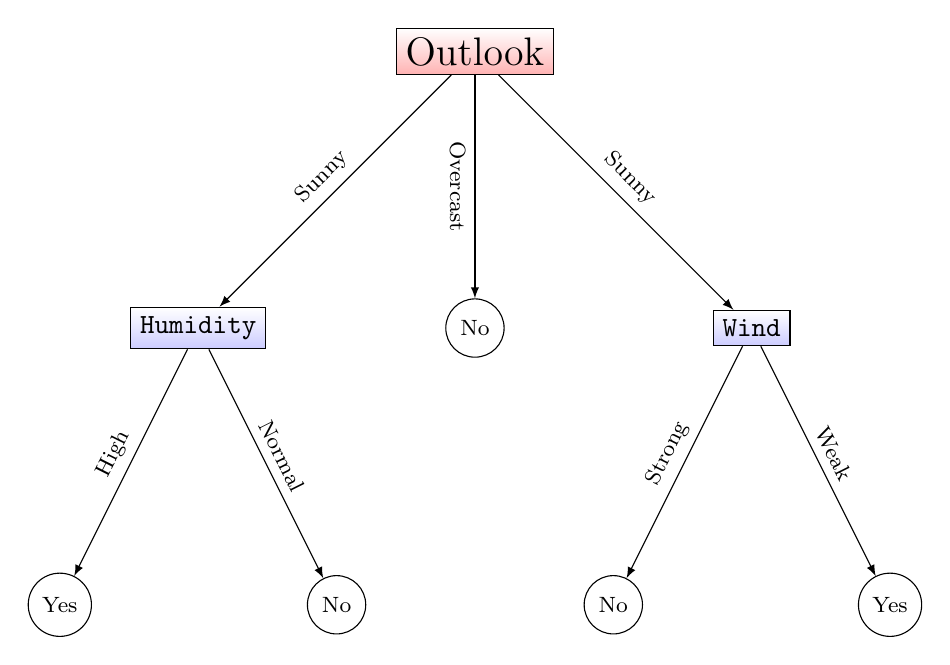
\begin{tikzpicture}
  [
    grow                    = down,
    sibling distance        = 10em,
    level distance          = 10em,
    edge from parent/.style = {draw, -latex},
    every node/.style       = {font=\footnotesize},
    sloped
  ]

\node [root] {Outlook}
    child { node [env] {Humidity}
       child { node [dummy] {Yes}
           edge from parent node [above] {High} }
       child { node [dummy] {No}
            edge from parent node [above] {Normal} }
    edge from parent node [above] {Sunny} }
    child { node [dummy] {No}
      edge from parent node [below] {Overcast} }
    child { node [env] {Wind}
       child { node [dummy] {No}
           edge from parent node [above] {Strong} }
       child { node [dummy] {Yes}
            edge from parent node [above] {Weak} }
    edge from parent node [above] {Sunny} };
\end{tikzpicture}
% \end{document}
					\label{fig:tree}
					\caption{Ví dụ về cây quyết định (Tham khảo từ trang 53 của \cite{mltextbook})}
				\end{figure}
				\par Cây quyết định (Decision Tree) là một mô hình học máy có giám sát, trong đó hàm mục tiêu được mô tả bằng một cây quyết định. Cây quyết định cũng có thể được biểu diễn lại dưới dạng một tập các luật giúp dễ đọc, dễ hiểu.
				\par Mỗi nốt của cây biểu diễn một thuộc tính. Mỗi nhánh xuất phát từ nốt đó thể hiện giá trị của thuộc tính đó. Một mẫu được phân loại trên cây quyết định bằng cách duyệt nó trên cây, bắt đầu từ gốc cho đến khi gặp giá trị phân loại (lá). 
				Cây quyết định ở Hình \ref{fig:tree} xét xem thử những buổi sáng thứ 7 nào sẽ có chơi quần vợt dựa trên các thuộc tính Outlook, Temperature, Humidity, Wind.
				\\Ví dụ mẫu (Outlook = Sunny, Temperature = Cold, Humidity = High, Wind = Strong) duyệt trên cây sẽ cho ra kết quả phân loại là mẫu âm (No). Cây quyết định này cũng có thể được biểu diễn lại thành luật, là hội của các tuyển:
				\begin{center}
					\begin{tabular}{l}				
						(Outlook = Sunny $\wedge$ Humidity = Normal)
						\\$\lor$ (Outlook = Overcast)
						\\$\lor$ (Outlook = Rain $\wedge$ Wind = Weak)
					\end{tabular}
				\end{center}											
			\subsubsection*{Giải thuật}		
				\par Phần lớn các giải thuật học trên cây quyết định (trong đó ID3 là giải thuật điển hình) đều theo hướng tiếp cận từ trên xuống, dùng giải thuật tham lam tìm kiếm trong không gian của tất cả các kết quả cây quyết định có thể xuất hiện. ID3 là giải thuật học cơ bản trên cây quyết định. Phần lớn các giải thuật học trên cây quyết định đều đi theo hướng tiếp cận của ID3, là sự mở rộng và nâng cấp của nó (trong đó có giải thuật C4.5).			
				\par Trong quá trình xây dựng cây từ trên xuống, ở mỗi bước cần xác định được thuộc tính nào là tốt nhất (được hiểu là thuộc tính phân loại hiệu quả nhất cho các mẫu) để làm gốc cho cây ở thời điểm đó. Sự lựa chọn thuộc tính tốt nhất được thực hiện nhờ vào độ đo \textit{Information Gain}.
				\begin{itemize}
					\item{Entropy: Là một hàm đo mức độ không thuần khiết (impurity) của tập mẫu, được sử dụng trong các giải thuật ID3, C4.5. Đối với các tập mẫu thuần khiết, giả sử tập mẫu gồm toàn mẫu âm hoặc dương (xét tập mẫu nhị phân), entropy sẽ bằng 0. Mặt khác đối với các tập mẫu "hỗn độn nhất", với số lượng mẫu âm và dương bằng nhau, entropy sẽ bằng 1. Giá trị của hàm entropy nói chung nằm trong đoạn [0,1] tùy theo số lượng mẫu của các loại. Ngoài ra, một số hàm đo khác (như Gini) có thể được sử dụng thay thể cho hàm Entropy.

					\begin{itemize}
						\item{Công thức Entropy:
						\\Xét tập S là tập mẫu nhị phân gồm các mẫu dương (+) và các mẫu âm (-). Khi đó:
						\begin{equation}					
						Entropy(S) \equiv -p_{(+)}log_{2}p_{(+)} - p_{(-)}log_{2}p_{(-)}
						\end{equation}}						
						\item{Ví dụ: Tập mẫu S gồm 14 mẫu nhị phân, trong đó có 8 mẫu dương và 6 mẫu âm.\\
						Tần số mẫu dương là: 8/14 \\
						Tần số mẫu dương là: 6/14 \\
					 	Khi đó entropy của tập S là:\\	
					 	\begin{align*}						
							Entropy(S) = -(8/14)log_{2}(8/14) - (6/14)log_{2}(6/14) = 0.985
						\end{align*}		
						}
					\end{itemize}}					
					\item{Information Gain: Là một hàm đo độ giảm entropy của tập mẫu khi phân đoạn nó trên một thuộc tính. Độ giảm entropy (độ giảm sự "không thuần khiết") càng cao thì phép phân đoạn đó càng hiệu quả.
					\begin{itemize}
						\item{Công thức Information Gain:
						\\Cho tập S và thuộc tính A. Khi đó: Information Gain của S trên A là:
						\begin{equation}
							\label{eq:gain}
							Gain(S,A) \equiv Entropy(S) - \sum_{v \in values(A)}\frac{|S_v|}{|S|}Entropy(S_v)
						\end{equation}}
						\item{Ví dụ: Tập mẫu S gồm 14 mẫu nhị phân, trong đó có 8 mẫu dương và 6 mẫu âm. 
						Thuộc tính A có 3 giá trị là A1, A2, A3. Thống kê cho thuộc tính A trên S như sau:
						\begin{table}[H]
							\centering
							\caption{Ví dụ tính Information Gain}
							\label{my-label}
							\begin{tabular}{|l|l|l|l|}
							\hline
							             & A = A1 & A = A2 & A = A3 \\ \hline
							Số mẫu dương & 2      & 3      & 4      \\ \hline
							Số mẫu âm    & 2      & 2      & 1      \\ \hline
							\end{tabular}
						\end{table}
						$\begin{aligned}							
							Entropy(S) = -(8/14)log_{2}(8/14) - (6/14)log_{2}(6/14) = 0.985				
						\end{aligned}$	
						\\
						$\begin{aligned}							
							Entropy(S_{A_1}) = -(2/4)log_{2}(2/4) - (2/4)log_{2}(2/4) = 1				
						\end{aligned}$	
						\\
						$\begin{aligned}							
							Entropy(S_{A_2}) = -(3/5)log_{2}(3/5) - (2/5)log_{2}(2/5) = 0.970
						\end{aligned}$
						\\
						$\begin{aligned}							
							Entropy(S_{A_3}) = -(4/5)log_{2}(4/5) - (1/5)log_{2}(1/5) = 0.722
						\end{aligned}$	
						\\						
						\begin{align*}							
					    	Gain(S,A) &= Entropy(S) - ((4/14)*Entropy(S_{A_1}) + (5/14)*Entropy(S_{A_2}) \\
					    	&+ (5/14)*Entropy(S_{A_3})) = 0.095					    	
						\end{align*}														
						}						
					\end{itemize}}					
				\end{itemize}
				\begin{figure}[H]
					\centering
					% \documentclass{article}

% \begin{document}
% \begin{figure}
	\noindent\fbox{
	    \parbox{\textwidth}{
	        ID3\textit{(Examples, Targetattribute, Attributes)
			\\Examples are the training examples. Targetattribute is the attribute whose value is to be
			predicted by the tree. Attributes is a list of other attributes that may be tested by the learned
			decision tree. Returns a decision tree that correctly classiJies the given Examples.}
			\begin{itemize}
				\item{Create a \textit{Root} node for the tree}
				\item{If all \textit{Examples} are positive, Return the single-node tree \textit{Root}, with label = +}
				\item{If all \textit{Examples} are negative, Return the single-node tree \textit{Root}, with label = -}
				\item{If \textit{Attributes} is empty, Return the single-node tree \textit{Root}, with label = most common value of \textit{Targetattribute} in \textit{Examples}}
				\item{Otherwise Begin
					\begin{itemize}
						\item{A $\gets$ the attribute from \textit{Attributes} that best* classifies \textit{Examples}}
						\item{The decision attribute for \textit{Root} $\gets$ A}
						\item{For each possible value, $v_i$, of A,
							\begin{itemize}
							\item{Add a new tree branch below \textit{Root}, corresponding to the test A = $v_i$}
							\item{Let \textit{$Examples_{v_i}$} be the subset of Examples that have value $v_i$ for A}
							\item{If \textit{$Examples_{v_i}$} is empty
								\begin{itemize}
									\item{Then below this new branch add a leaf node with label = most common value of \textit{Targetattribute} in \textit{Examples}}
									\item{Else below this new branch add the subtree ID3(\textit{$Examples_{v_i}$ (Targetattribute, Attributes - \{A\}})}
								\end{itemize}}
							\end{itemize}}
					\end{itemize}}			
				\item{End}
				\item{Return Root}
			\end{itemize}
			}
		} 	
% \end{figure}
% \end{document}
					* The best attribute is the one with highest information gain, as defined in Equation 
					\ref{eq:gain}
					\caption{Giải thuật ID3 trong cây quyết định (Tham khảo từ trang 59 của \cite{mltextbook})}
					\label{fig:id3}
				\end{figure}
			\subsubsection*{Vấn đề Quá vừa dữ liệu}
				\par Giải thuật ở Hình \ref{fig:id3} là hợp lý trong một số trường hợp, nhưng thực tế nó có thể dẫn đến hiện tượng \textit{Quá vừa dữ liệu (Overfitting data)}. Điều này xảy ra là bởi vì giải thuật này chỉ cố gắng xây dựng cây đủ để phân loại đúng tập huấn luyện, \textit{Quá vừa dữ liệu} sẽ xảy ra nếu dữ liệu trong tập huấn luyện bị nhiễu hoặc chứa quá ít mẫu để có thể xấp xỉ đúng hàm mục tiêu.
				\par Một phương pháp phổ biến được sử dụng để giải quyết hiện tượng này là cho phép cây bị \textit{Quá vừa dữ liệu}, nhưng sau đó cắt tỉa (post-pruning). Trong phương pháp này, tập huấn luyện được chia ra làm hai, một cho huấn luyện (training set) và một cho kiểm thử phép cắt tỉa (validation set). Cây sẽ được xây dựng dựa trên tập huấn luyện trước, có 2 hướng giải quyết vấn đề cắt tỉa:
				\begin{itemize}
				\item{Cắt tỉa giảm lỗi (reduced error pruning): Cân nhắc từng nốt của cây, và thực hiện cắt tỉa cây con có gốc là nốt đó. Cây sau phép cắt tỉa này được đánh giá độ chính xác dựa vào tập kiểm thử, nếu độ chính xác không thấp hơn cây trước phép cắt tỉa thì cho phép cắt tỉa. Việc cắt tỉa được lặp lại với các nốt không làm giảm độ chính xác của cây cho đến khi không còn lựa chọn nào.}
				\item{Cắt tỉa theo luật (rule post-pruning): Đây là phương pháp được sử dụng trong giải thuật C4.5, bao gồm các bước:
					\begin{itemize}
						\item{Xây dựng cây từ tập huấn luyện}
						\item{Chuyển cây thành một tập các luật}
						\item{Cắt tỉa điều kiện (precondition) trong các luật sao cho độ chính xác không giảm (đối với C4.5, tính toán độ chính xác trên toàn bộ tập huấn luyện)}
						\item{Sắp xếp tập các luật cuối cùng (sau khi cắt tỉa xong) theo độ chính xác và sử dụng các luật này để phân loại cho các mẫu mới (unseen data).}
					\end{itemize}}				
				\end{itemize}

	\section{Phương pháp đề xuất}
		\subsection{Nội dung bài toán}
		\subsection{Tổng quan quy trình}
			\begin{figure}[H]
				\centering				
				% Author: Rasmus Pank Roulund
%\documentclass{minimal}
%\usepackage{tikz}
%\usepackage[utf8]{vietnam}

%\begin{document}
\usetikzlibrary{arrows,chains,positioning,scopes}

\tikzset{
    block/.style={draw,text width=4em,minimum height=6.5em,minimum width=4em,align=center},
    arrow/.style={->, thick}
}
\begin{tikzpicture}
  {[start chain]
        \node[block,on chain] (N1) {Thu thập dữ liệu thô};
        \node[block,on chain,join=by {arrow},right=0.7cm of N1] (N2) {Tiền xử lý dữ liệu};
        \node[block,on chain,join=by {arrow},right=0.7cm of N2] (N3) {Trích xuất cụm danh từ};
        \node[block,on chain,join=by {arrow},right=0.7cm of N3] (N4) {Gán nhãn dữ liệu};
       \node[block,on chain,join=by {arrow},below=0.7cm of N4] (N5) {Trích xuất thuộc tính};
       \node[block,on chain,join=by {arrow},left=0.7cm of N5] (N6) {Tạo tập huấn luyện và tập kiểm tra};
       \node[block,on chain,join=by {arrow},left=0.7cm of N6] (N7) {Áp dụng giải thuật học máy};
       \node[block,on chain,join=by {arrow},left=0.7cm of N7] (N8) {Đánh giá};
    }
      
  \end{tikzpicture}
%\end{document}
			\end{figure}
		\subsection{Tiền xử lý dữ liệu}
		\subsection{Trích xuất cụm danh từ}
		\subsection{Trích xuất thuộc tính}
		\subsection{Tạo bộ phân loại}		
		\subsection{Gom cụm các đồng tham chiếu}	

	\section{Thực nghiệm và đánh giá}

	\section{Tổng kết}		

\renewcommand{\refname}{Tham khảo} 

%----------REFERENCES-------------------
\begin{thebibliography}{30}

	\bibitem{mainpaper} 
	Ding, Xiaowen and Bing Liu. 2010.
	\textit{Resolving Object and Attribute Coreference in Opinion Mining}. 
	Proceedings of International Conference on Computational Linguistics (COLING-2010). 2010.
	 
	\bibitem{findfeatures1} 
	Minqing Hu and Bing Liu. 2004.
	\textit{Mining and Summarizing Customer Reviews}.
	Proceedings of the ACM SIGKDD International Conference on Knowledge Discovery and Data Mining (KDD-2004), Aug 22-25, 2004, Seattle, Washington, USA.

	\bibitem{findfeatures2} 
	A-M. Popescu and O. Etzioni. 2005. 
	\textit{Extracting product features and opinions from reviews}.
	EMNLP’05.

	\bibitem{corefdef}
	Joseph F. Mccarthy. 1996.
 	\textit{A trainable approach to coreference resolution for information extraction}.

 	\bibitem{sentiment}
 	Bing Liu. 2010.
 	\textit{Sentiment Analysis and Subjectivity}. A chapter in 
  	Handbook of Natural Language Processing, Second Edition, 
  	(editors: N. Indurkhya and F. J. Damerau), 2010.

  	\bibitem{comparative1}
  	Nitin Jindal and Bing Liu. 2006.  
  	\textit{Identifying Comparative Sentences in Text Documents}. 
   	Proceedings of the ACM SIGIR International Conference on 
   	Information Retreival (SIGIR-06), 2006.

   	\bibitem{comparative2}
	G. Ganapathibhotla and B. Liu. 2008.
	\textit{Identifying Preferred Entities in Comparative Sentences}.
	Proceedings of the International Conference on Computational Linguistics, COLING, 2008.

	\bibitem{mltextbook}
	Tom Mitchell, McGraw Hill, 1997.
	\textit{Machine Learning}.
	Publisher: McGraw-Hill Science/Engineering/Math; (March 1, 1997). ISBN-0070428077.	
 
\end{thebibliography}	

\end{document}
